\documentclass{article}
\usepackage{graphicx} % Required for inserting images
\usepackage{hyperref}
\hypersetup{
    colorlinks=true, % Set this to true to remove the border
    linkcolor=black, % Color for internal links
    citecolor=black, % Color for citations
    }
\usepackage{listings}
\usepackage{blindtext}
\usepackage{geometry}
\geometry{margin=25mm}
\begin{document}

\section{Encoding Software}
\label{sec: encoder}

To encode the loss less images into the respective codec for the experiment, several encoder where used.
\subsection{AVIF, JPEG and WebP}
For those encoders the python package pillow-avif-plugin and pillow was used. The additional pillow plugin can be installed via pip install pillow-avif-plugin. To encode a lossless image, the image is opened and save with a specific quality as seen in listing \ref{avif_1}. The quality parameter ranges from 1(lowest) to 100(highest). It is important to set the specific file extension for the software to
know in which codec the image needs to be encoded.
\begin{lstlisting}[label={avif_1}, language=Python, caption=Encode AVIF\, JPEG and WebP]
image = Image.open(image_path)
image.save(outputPath, quality=q)
\end{lstlisting}

\subsection{BPG}
To encode the images in BPG the Linux distribution from Fabrice Bellard's website (https://bellard.org/bpg/) was used. As seen in listing \ref{bpg_1} the output path is given after the -o argument and the specific quality after the -q argument. The quality parameter ranges from 51(lowest) to 0(highest). The last argument that needs no specific indicator is the original image.

\begin{lstlisting}[label={bpg_1}, language=Python, caption=Encode BPG]
os.system('bpgenc -o ' + outputPath + \
    ' -q ' + str(int(maxQ - q)) + \
    ' ' + image_path)
\end{lstlisting}

\subsection{HEIC}
Same as with the AVIF codec HEIC is also supported in a python package. For this codec the package pillow\_heif which can be installed with pip pillow-heif. The quality parameter ranges from 1(lowest) to 100(highest).
How the image can be encoded in HEIC is shown in listing \ref{heic_1}.

\begin{lstlisting}[label={heic_1}, language=Python, caption=Encode HEIC]
image = pillow_heif.from_pillow(Image.open(image_path))
image.save(outputPath, quality=q)
\end{lstlisting}

\subsection{JPEG2000}
For the JPEG standards JPEG itself provides software to encode images. In the experiment the libopenjp2 was used. This library is in the Linux package manager and can be installed with apt-get install libopenjp2-tools. The quality parameter which ranges from 1(lowest) to 1000(highest) is given to the software with the -r parameter. An example how this can be done in Python is shown in listing \ref{jpeg2k_1}.
\begin{lstlisting}[label={jpeg2k_1}, language=Python, caption=Encode JPEG 2000]
subprocess.call('opj_compress -o ' + outputPath + \
                ' -r ' + str(int(maxQ - q)) + \
                ' -i ' + image_path,
                stdout=subprocess.DEVNULL,
                stderr=subprocess.DEVNULL,
                shell=True)
\end{lstlisting}

\subsection{JXL}
For JPEG XL the JPEG organization also provides a package which can be installed in Linux. For that encoder the libjxl (apt install libjxl-devtools) was used. The quality parameter ranges from 1(lowest) to 100 (highest) and an example to encode a image is shown in \ref{jxl_1}
\begin{lstlisting}[label={jxl_1}, language=Python, caption=Encode JPEG XL]
subprocess.call(['cjxl', image_path, outputPath,
                 '--quiet', '-q', str(q)])
\end{lstlisting}
\subsection{JXR}
For JXR the package libjxr-devtools was used. This includes a specific encoder and decoder app. The quality ranges from 0(lowest) to 1(highest). Here floating point numbers need to be used for quality.
An example how to encode a image with jxr is shown in \ref{jxr_1}. In addition to the quality parameter jxr also support quantization, although this results in very good compression rate, the image quality is affected drastically.
\begin{lstlisting}[label={jxr_1}, language=Python, caption=Encode BPG]
os.system('JxrEncApp -q ' + q_str + \
            ' -o ' + output_path + \
            ' -i ' + tif_path)
\end{lstlisting}

\newpage
\section{Achieving Fixed Filesize Compression Through Binary Search Algorithm}
\label{sec: filesize}

The primary objective was to attain a consistent and fixed filesize for the encoder discussed in chapter \ref{sec: encoder}. To achieve this goal efficiently, we devised a binary search algorithm, strategically designed to conserve computational resources and time. This algorithm, when coupled with the encoders enabled us to successfully compress the original images while maintaining a specified filesize. The results are graphically represented in image \ref{fig: fsize_comparison}, which displays boxplots illustrating the distribution of the encoder performances for targeting file size 32kB.

\begin{figure}[h!]
	\centering
	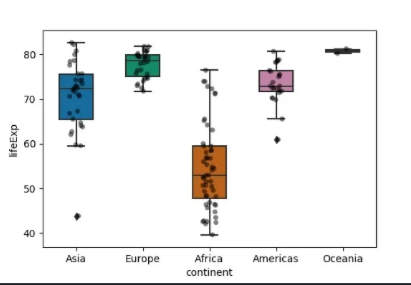
\includegraphics[width=8cm]{filesize_comparison.png}
	\caption{Archived filesizes for used encoder}
	\label{fig: fsize_comparison}
\end{figure}

\noindent
To ensure the proper functioning of the employed encoder, we conducted calculations of Peak Signal to Noise Ratio (PSNR) and generated plots depicting its relationship with the achieved compression rates. To maintain clarity in the plots, we utilized JPEGXR with its default overlapping parameter (1).

\begin{figure}[h!]
	\centering
	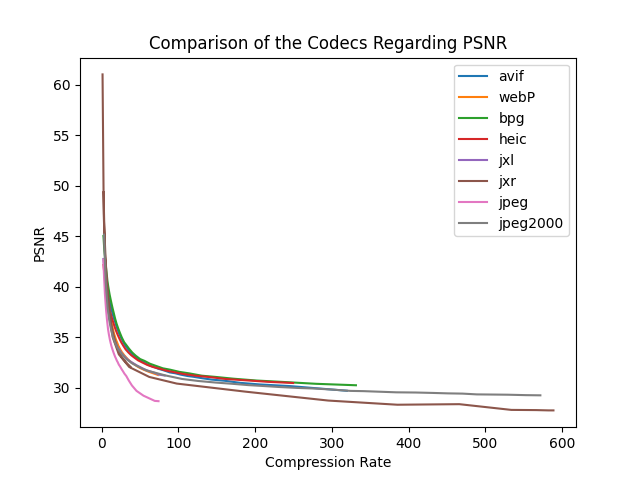
\includegraphics[width=8cm]{psnr.png}
	\caption{PSNR comparison of the used codecs}
	\label{fig: psnr_comparison}
\end{figure}

\noindent
As anticipated, the results presented in plot \ref{fig: psnr_comparison} affirm that the plain JPEG encoder consistently yields in reduced-quality images when operating at lower compression rates.
The driving motivation behind this attempt was to intentionally introduce diverse encoding artifacts into the compressed images for later train a model and classify the used image encoder.
\newpage

\section{RESNET explanation}
Residual Networks are deep learning models, that where developed by Kaiming He, Xiangyu Zhang, Shaoqing Ren, and Jian Sun. This networks enable easier training of deep learning models. For an explicit explanation on how a ResNet works see \cite{he2015deep}.

@misc{he2015deep,
      title={Deep Residual Learning for Image Recognition}, 
      author={Kaiming He and Xiangyu Zhang and Shaoqing Ren and Jian Sun},
      year={2015},
      eprint={1512.03385},
      archivePrefix={arXiv},
      primaryClass={cs.CV}
}

\subsection{Training without transfer learning}

The idea behind training the network from scratch is that the network would be more tailored to the given task since it has no previous information stored in the network. This contrasts with transfer learning since there prior information is present.
\newline

\noindent
\textbf{Dataset Details:}

\noindent
To train the network the DIV2K training and validation dataset was used. The dataset contains 800 train images and 100 test images. Since the images had different dimensions, we first had to crop them to specific in this case 512x512. Afterwards we compressed the images to specified file sizes as described in \ref{sec: filesize}. This leads to 10 classes – one for each compression algorithm – for each file size category. We trained the network by using the images that were compressed to a file size of 25kB.
\newline

\noindent
\textbf{Training Details:}

\noindent
For the self-trained network, we used an Adam Optimizer with a learning rate of 1e-4 and a weight decay of 1e-4. As a loss function Cross entropy was used. To be able to match the output of the network to the 10 classes used we replaced the final fully connected layer in the Resnet architecture with one that outputs the 10 codec classes.

\noindent
In the first iteration we trained the network on the original cropped 800 images per class. This leads to 8000 images available for the network to train. With that amount there was little progress during the first epochs. To be able to train on a larger dataset we then cropped the corners of each image to 512x512 to get 5x the number of usable images. This lead to 4000 images per class for the network to train.

\noindent
After 10 epochs of training, we achieved a validation accuracy of 57,6 percent. For 10 epochs this is lower than the results we got for the transfer learning approach. However, if one would increase the number of epochs, we expect to reach the same levels of accuracy since the only defencemen is that the pretrained network has a preferable starting position compared to the one without transfer learning. This can be shown by changing the starting seed to something different leading to only 10 percent accuracy after 10 epochs.

\subsection{Transferlearning}
For this approach the ResNet18 model was used as a baseline. To adjust this pretrained model for the requirements of the experiment, the output layers where reconfigured to represent the 8 different codecs in which the images where encoded.
In addition the model uses just 224x224 images as inputs, thus the encoded images where center cropped to fit that size.



\noindent
Then the model was trained over 10 epochs on 4000 test images. The learning rate was set to 0.001 with a momentum of 0.9 due to the model being already trained on a huge data set and in the experiment just the adjustment for the codec artifacts should be added. For the whole implementation see appendix.

\section{Results}
\label{Results}
A mixed model was developed by training the model with images of filesizes 5, 10, 17, 25 and 32. This resulted in 4500 images (512x512) for each codec. The considered dataset has only 900 images. To compare the filesize models with the mixed model, the filesize models need the same amount of input images as the mixed model. Therefore, each image of the dataset was cropped into five images to get an amount of 4500 images for the training and testing.

\section{Performance}
For the classification each model was evaluated with each filesize. The result is represented in the figure \ref{fig: acc_comparison}.

\begin{figure}[h!]
	\centering
	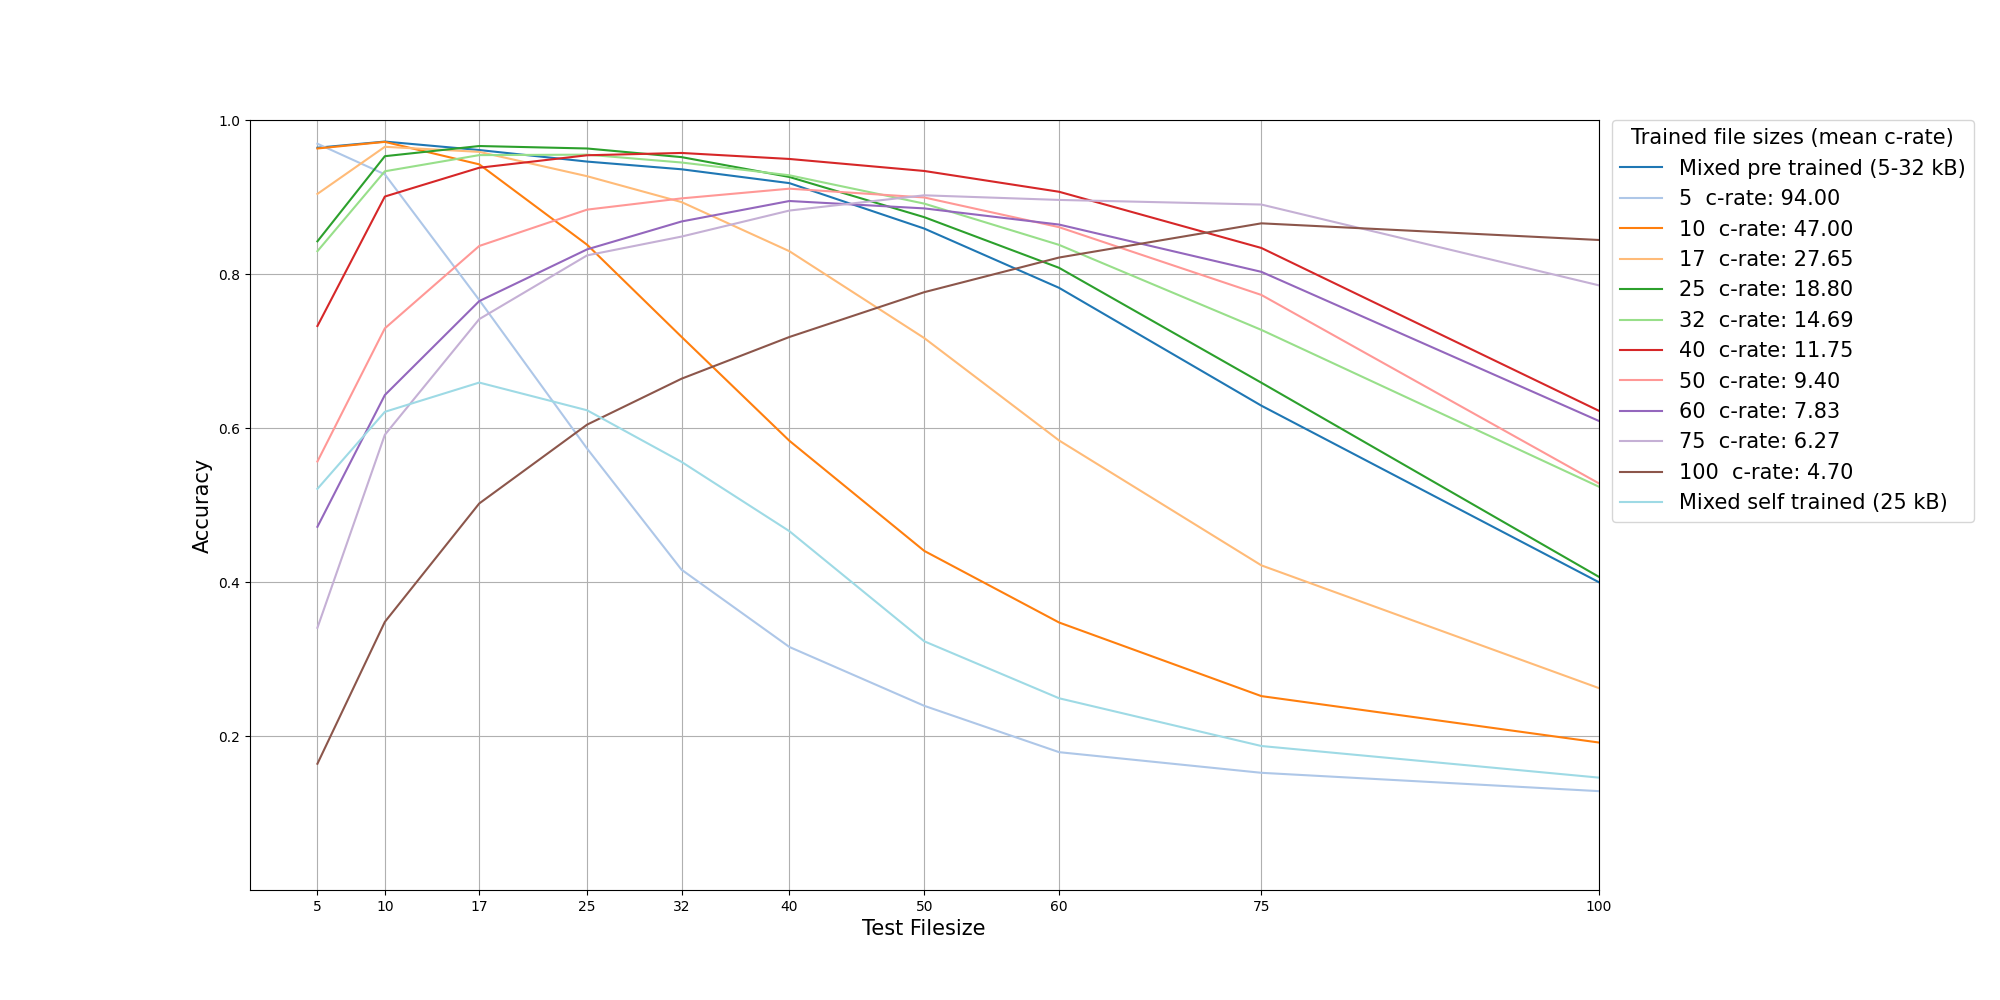
\includegraphics[width=12cm]{accuracy_comparison.png}
	\caption{Accuracy Comparison}
	\label{fig: acc_comparison}
\end{figure}

\noindent
The self trained model showed an accuracy over all filesizes of 10 percent. With ten different codecs, random guessing would lead to the same result as this model. For the self trained model 40000 images where used. The pretrained model was already trained on 1,2 million images. Therefore, the self trained model would need much more images to get a better performance. With only 2400 images used for training, this model represents the worst model for the classification task.

\noindent
The models trained with the filesizes 60, 75 and 100 have a low accuracy for small filesizes and increase for bigger filesizes. Small filesize images have more artifacts, which are not taken into account in this models. For that reason the models of 60, 75 and 100 filesize could only be used to classify codecs with the same filesizes.

\noindent
The smaller filesize models have their peaks around the filesizes they were trained on. However, for the images with less than 40kB this models have an accuracy of about 95 percent. For the bigger filesizes the accuracy is decreasing. The bigger filesizes have less artifacts in the images and also many codecs get the maximum quality after 60kB, which explains the decrease of accuracy for this models.

\noindent
An assumtion was that the mixed model would lead to the best result because of considering different filesizes for the model. As the figure \ref{fig: acc_comparison} shows, almost every small filesize model has a better performance than the mixed model. 

\noindent
For classifying images with the given filesizes the model trained with 40kB would lead to the best result. However, for smaller filesize images (\textless 50kB) the model trained with 32kB images would be the right choice because of the bigger accuracy for 5kB images.

\section{Loss function}

\begin{figure}[h!]
    \centering
    \begin{minipage}{0.7\textwidth}
        \centering
        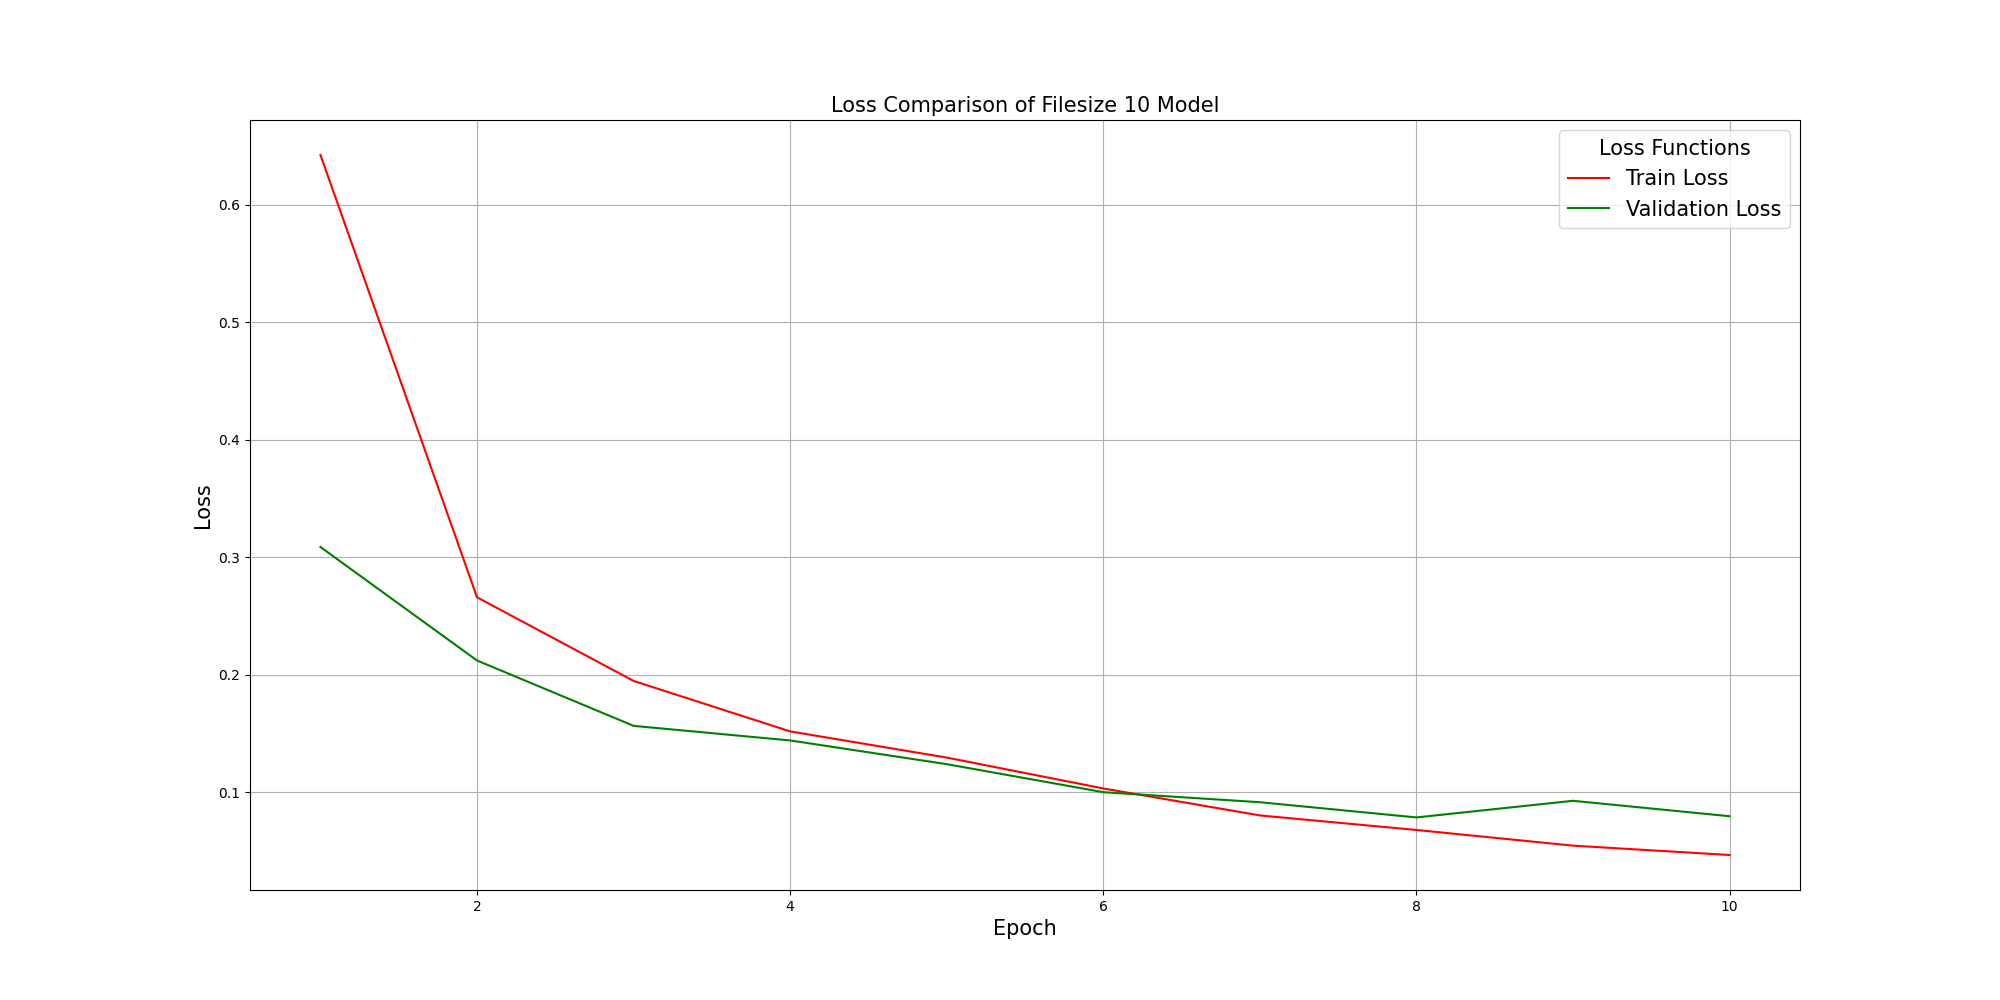
\includegraphics[width=1\linewidth]{loss_comparison_filesize_10.png}
        \caption{Loss of model with filesize 10}
        \label{fig:loss_comparison_filesize_10}
    \end{minipage}\hfill
    \begin{minipage}{0.7\textwidth}
        \centering
        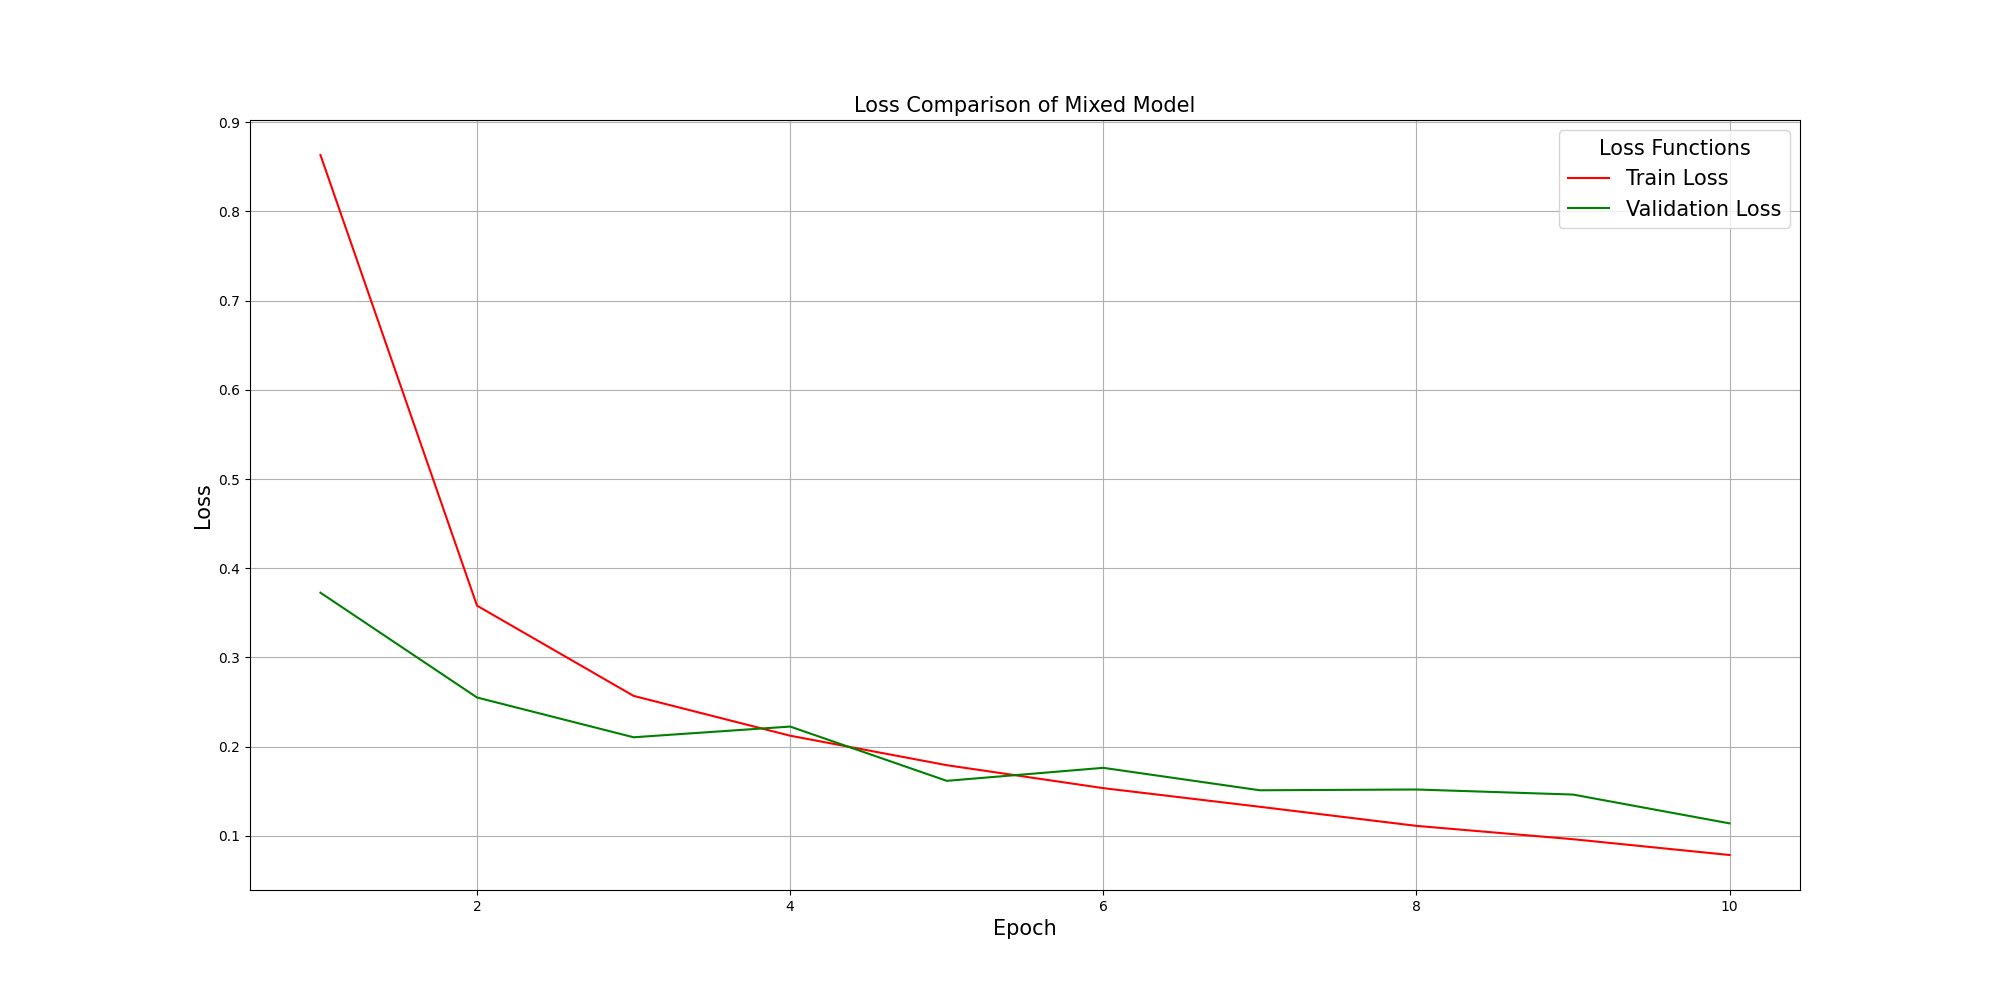
\includegraphics[width=1\linewidth]{loss_comparison_mixed.png}
        \caption{Loss of mixed model}
        \label{fig:loss_comparison_filesize_mixed}
    \end{minipage}
\end{figure}

\noindent
In the figure \ref{fig:loss_comparison_filesize_10} and \ref{fig:loss_comparison_filesize_mixed} the loss over ten epochs is represented. After 10 epochs the loss is already minimal, therefore further training would not make a significant change. The other nine models show a similar behavior as figure \ref{fig:loss_comparison_filesize_10} shows.

\end{document}
